\section{Builder}

Quando é necessário criar objetos  
complexos, o padrão Builder retira a 
responsabilidade da criação do objeto e 
a coloca em classes separadas. Dessa forma, 
um mesmo processo de criação pode criar 
representações diferentes desse mesmo 
objeto. Essas novas classes devem ser 
independentes de todas as partes que 
compõem o objeto que será criado.

A figura \ref{builder_struct} apresenta 
a estrutura do Builder, onde a interface 
Builder representa uma classe responsável 
por criar uma parte de um objeto. A classe 
ConcreteBuilder, do tipo dessa interface, 
implementa os métodos de construção de 
uma parte do tipo Product. A classe Director 
é responsável por chamar o método de criação 
das classes que criam cada parte do objeto 
complexo.

\begin{figure}[htb]
	\caption{\label{builder_struct}Estrutura do Builder}
	\begin{center}
	    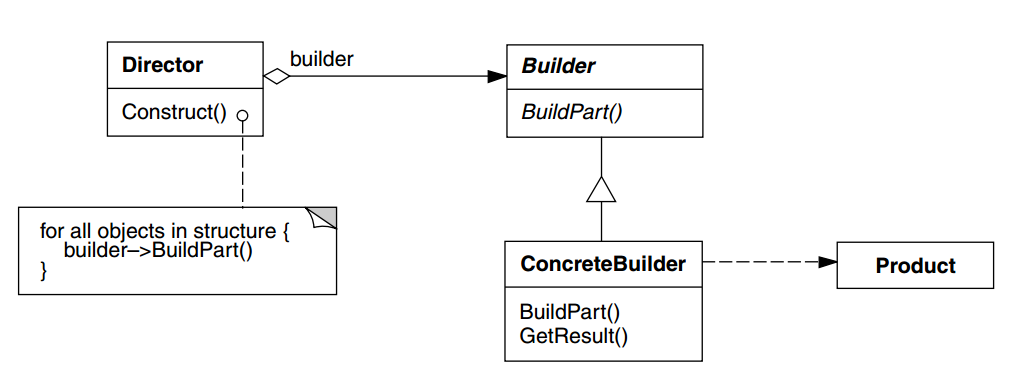
\includegraphics[scale=0.4]{5_padroes-contexto-funcional/5.1_criacionais/5.1.3_builder/diagram.png}
	\end{center}
\end{figure}

\subsection*{Exemplo Orientado a Objetos}

Como exemplo, podemos observar um leitor de 
documentos do tipo RTF (\textit{Rich Text Format}), 
que deve permitir a conversão de documentos RTF 
para outros formatos, como texto em ASCII ou em um 
\textit{widget} de texto que pode ser editado de 
forma iterativa. Como a quantidade de formatos 
possíveis é grande, deve ser possível adicionar 
novos formatos sem que seja necessário modificar 
a classe do leitor de documentos RTF. 

O diagrama de classes apresentado na imagem 
\ref{builder_exemplo} demonstra o uso do padrão 
Builder para esse exemplo. Para cada formato possível 
de conversão, uma nova classe Builder é criada. 
As classes ASCIIConverter, TeXConverter e 
TextWidgetConverter representam, respectivamente, 
os \textit{builders} para os conversores para texto 
em ASCII, LaTeX e \textit{widget} de texto. A classe 
RTFReader chama as operações de construção 
apenas dos conversores desejados. O exemplo de 
implementação dessa abordagem é apresentado no 
código \ref{oobuilder}.

\begin{figure}[htb]
	\caption{\label{builder_exemplo}Exemplo de Builder}
	\begin{center}
	    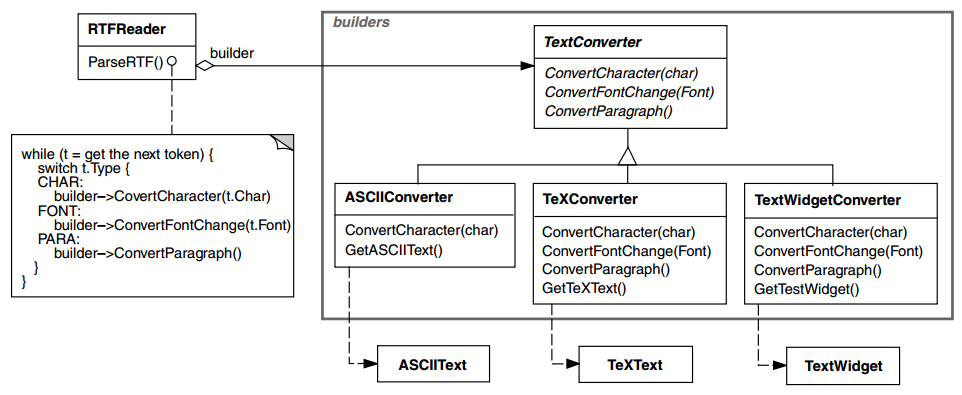
\includegraphics[scale=0.4]{5_padroes-contexto-funcional/5.1_criacionais/5.1.3_builder/exemplo_builder.png}
	\end{center}
\end{figure}

\begin{lstlisting}[caption={Builder Orientado a Objetos},label=oobuilder]

	trait TextConverter {
		def ConvertCharacter(char : Char)
		def ConvertFontChange(font : String)
		def ConvertParagraph()
	} 

	class TextConverter {
		
		private var asciiText : ASCIIText

		def ConvertCharacter(char : Char){
			// Conversão para ASCIIText
		}

		def GetASCIIText() : ASCIIText {
			return this.asciiText
		}
	} 

	class TeXConverter {
		
		private var texText : TeXText

		def ConvertCharacter(char : Char){
			// Conversão para TeXText
		}

		def ConvertFontChange(font : String) {
			// Conversão para TeXText
		}

		def ConvertParagraph() {
			// Conversão para TeXText
		}

		def GetTeXText() : TeXText {
			return this.texText
		}
	} 

	class TextWidgetConverter {
		
		private var textWidget : TextWidget

		def ConvertCharacter(char : Char){
			// Conversão para TextWidget
		}

		def ConvertFontChange(font : String) {
			// Conversão para TextWidget
		}

		def ConvertParagraph() {
			// Conversão para TextWidget
		}

		def GetTeXText() : TextWidget {
			return this.textWidget
		}
	} 

	class RTFReader() {

		private var builder : Builder

		def ParseRTF() {
			// ...

			for(t <- tokens) {
				t.Type match {
					case CHAR => builder.ConvertCharacter(t.Char)
					case FONT => builder.ConvertFontChange(t.Font)
					case PARA => builder.ConvertParagraph()
				}
			}

			// ...
		}

	}


\end{lstlisting}

\subsection*{Contexto Funcional}


\begin{lstlisting}[caption={Builder Funcional},label=fpbuilder]
    

    
\end{lstlisting}